\chapter{データプレーン高速化に伴う課題}
\label{issue}
本章では\ref{related:a-dplane}で述べたような技術を利用した際に生じる課題について述べる.
\section{高速パケット処理フレームワークの課題}

\label{issue:dplane}

\section{コントロールプレーン資産の再利用不可能性の弊害}
\label{issue:cplane}
コントロールプレーン資産を

% \subsection{概要}
% SIIT-DCとは,ステートレスIP/ICMP変換アルゴリズム\cite{RFC7915}を利用して,IPv4インターネット・ネットワークからのアクセスをIPv6シングルスタックネットワーク上のホストに提供するためのネットワークデザインである.2016年にIETF IPv6 Operations WG\footnote{IPv6ネットワークの運用要件や関連する技術仕様の策定を行うワーキンググループ.\url{https://datatracker.ietf.org/wg/v6ops/about/}}での議論を基にRFC7757として標準化された\cite{RFC7755}.


% \subsection{用語}
% \label{issue:siit-dc:terms}
% SIIT-DCで利用される用語,及び特徴的な役割を有する機器・技術について述べる.

% \subsubsection{SIIT(Stateless IP/ICMP Translation Algorithm)}
% SIITとはIPv4/IPv6トランスレーションに用いられるプロトコル変換機能の略称である.RFC2765\cite{RFC2765}で初めて標準化され,その後RFC6145\cite{RFC6145}により一部の仕様が実運用のユースケースに合わせて変更された.現在はIPv6拡張ヘッダーを扱う機構などが追加されたRFC7915\cite{RFC7915}が現行の標準仕様である.

% \subsubsection{BR(Border Relay)}
% BRとは,SIIT-DCネットワークにおいてIPv4インターネットとIPv6ネットワークとの間でSIITによるIPv4/IPv6トランスレーションを行う機器もしくは他の役割を有する機器の一機構である.
% IPv4インターネットとIDC内のIPv6シングルスタックネットワークの各境界部に所在し,後述するEAMTを参照した1:1のアドレス変換を行う.IDCネットワークにIPv4インターネットとの接続点が複数ある場合,接続点ごとに最低一つのBRを配備する.

% \subsubsection{ER(Edge Relay)}
% ERとは,IDC内のIPv4ネットワークとIPv6ネットワーク間での多:多のIPv4/IPv6トランスレーションを行う機器である.

% SIIT-DCではそのオプションとして,IPv4ネットワーク内のIPv4しか利用出来ないホストが,SIIT-DCを利用してIPv4サービスを提供するユースケースをサポートするSIIT-DC Dual Translation Mode\cite{RFC7756}が定義されており,ERはその中での利用が想定されている.

% 通常,ERが有する後述のEAMTはIDCネットワーク内のIPv4ネットワークアドレスと,そのIPv4ネットワークを示すIPv6サービスアドレスにより構成される.

% \subsubsection{IPv4サービスアドレス}
% IPv4サービスを提供するIPv6シングルスタックネットワークに属するホストに割り当てるIPv4アドレス(群)をIPv4サービスアドレスと呼称する.
% このアドレス宛に送信されたパケットは,BR/ERによって対応するIPv6サービスアドレスに変換される.

% なお,IPv4サービスアドレスはIPv4インターネットに経路広告されている必要がある.

% \subsubsection{IPv6サービスアドレス}
% ER/BRを介してアプリケーションやホストに割り当てられたIPv6アドレス(群)をIPv6サービスアドレスと呼称する.
% IPv4クライアントはSIIT-DCのアーキテクチャをを通じて,このIPv6サービスアドレスが割り当てられたホストと通信することが出来る.

% \subsubsection{変換プレフィックス}
% \label{issue:siit-dc:translation-prefix}
 
% 変換プレフィックス(Translation Prefix)とは,全てのIPv4アドレスをマッピングするために用いられる,プレフィックス長が96bitのIPv6ネットワークプレフィックスである\cite{RFC6052}.IANAによって主にWKP(Well Known Prefix)として64:ff9b::/48が予約\cite{RFC8215,IANA_allocation_v6}されているが,運用者の裁量でISP自身に割り当てられたNSP(Network Specific Prefx)\footnote{主にRIRから割り当てられたIPv6 Global Unicas Addressを指す.}を利用する事ができる.

% IPv4アドレスとIPv6アドレスの間で変換を実行する際に,BR/ERは変換前のIPヘッダーのアドレスフィールドを、変換プレフィックスが挿入・削除された状態に書き換える。

% なおSIIT-DCネットワークにおいて,変換プレフィックス宛のパケットは各BR/ERのIPv6インターフェース宛にIGP(Interior Gateway Protocol)などで経路広告される必要がある.

% \subsubsection{EAM(Ecplicit Address Mapping)/EAMT(Ecplicit Address Mapping Table)}
% EAMとは,EAMアルゴリズム\cite{RFC7757}によって結びつけられたIPv4サービスアドレスとIPv6サービスアドレスのペアを表す.

% EAMにおいて,それぞれ同数のIPv4サービスアドレスとIPv6サービスアドレスによって構成される.標準では結び付けられたIPv6サービスアドレスがIPv4サービスアドレスより多い状態が想定されているが,IPv6サービスアドレスのホスト部が若いものから優先して変換するため,余剰分のアドレスは無視される.

% また,BR及びERが変換を行う際に参照するEAM群が記録されたテーブルをEAMTと定義している.以後EAMTもしくは変換テーブルと呼称する.



% \subsection{ネットワーク設計}
% \label{issue:siit-dc:network}
% \begin{figure}[h]
%     \begin{center}
%       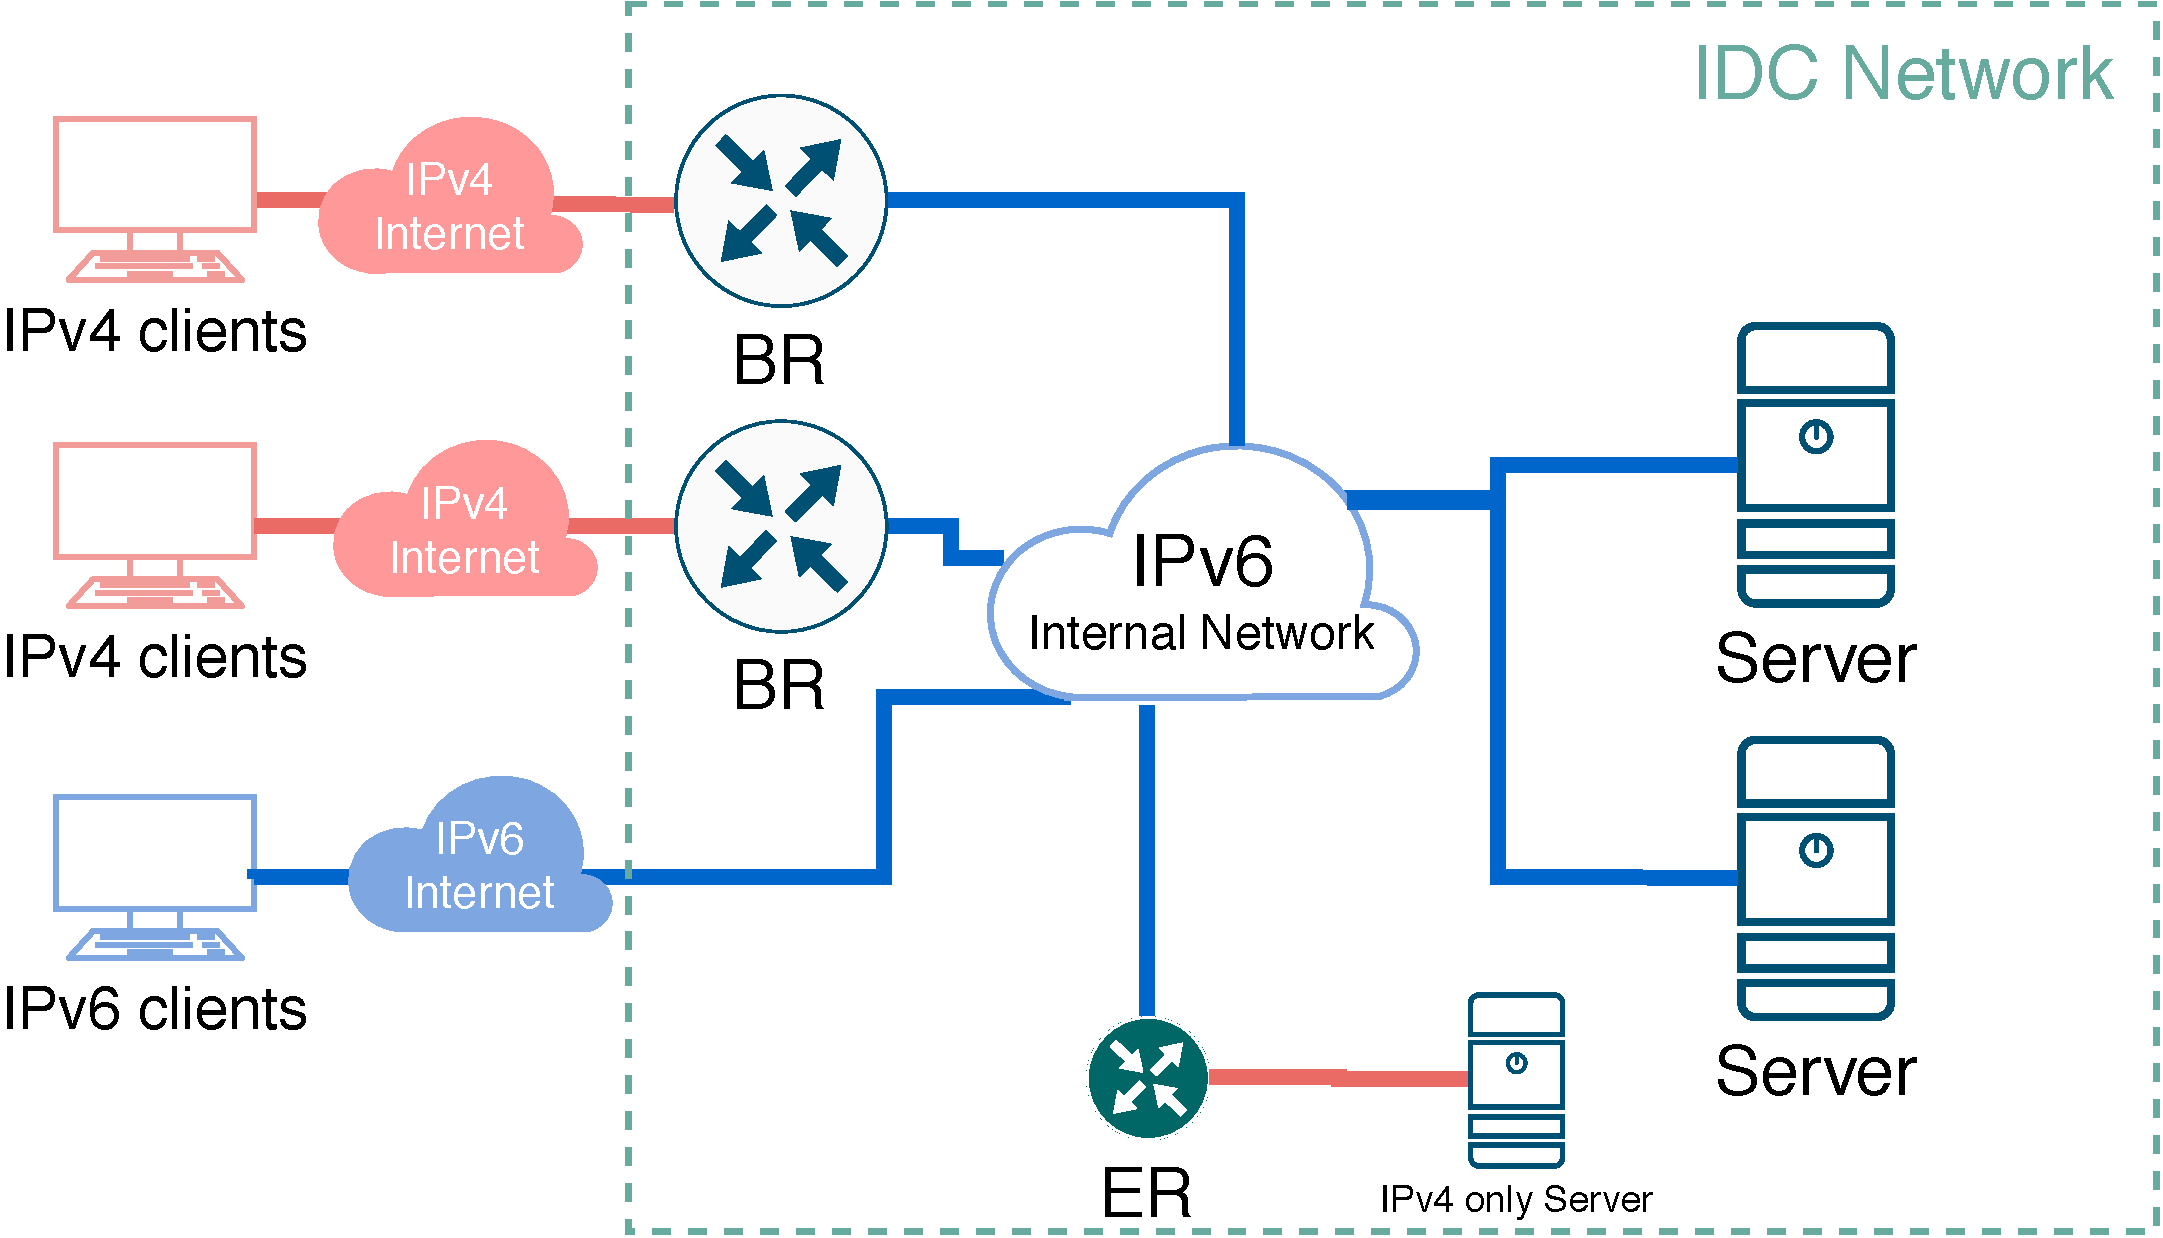
\includegraphics[width=12cm,pagebox=cropbox,clip]{img/siit-dc-network.pdf}
%     \end{center}
%     \caption{SIIT-DC ネットワーク}
%     \label{fig:siit-dc_network}
% \end{figure}
% 基本的なSIIT-DCネットワークを図\ref{fig:siit-dc_network}に示す.

% BRはIPv4インターネットとの各接続点に配置される.各IPv4サービスアドレスは自組織のアドレスとして,IPv4インターネットに経路広告される必要がある.

% SIIT-DCネットワークでは,変換プレフィックス宛のパケットはBRに対してルーティングされる.
% BRが複数ある場合,BRがネットワークプロトコルに利用する変換プレフィックスを別個に用意するか,同一の変換プレフィックスを各BRにエニーキャスト\cite{RFC4786}によってルーティングさせる.エニーキャストを使用した場合,BRの障害時には別のBRへとトラフィックを迂回させることが可能である.

% ERはIDC内のIPv4ネットワークとの接続点に配置され,IPv4のみを持つホストがIDC内のIPv6ネットワークを介してIPv4インターネットにサービス提供を行う場合に利用される.


% \subsection{SII-DCのメリット}
% \label{issue:siit-dc-merit}
% SIIT-DCを用いたIPv4サービスの提供によるメリットとして,以下の点が挙げられる,

% \subsubsection{デプロイメントが容易}
% SIIT-DCでは,IDCのIPv6ネットワークとIPv4インターネットとの接続点にBRを設置を行うのみにより,基本的なIPv4サービスの提供が可能である.
% そのためIDCのネットワークトポロジに限定されないシンプルなIPv4サービス提供が期待できる.

% \subsubsection{アドレス単位でのIPv4アドレスの効率的な利用が可能}
% 通常のIPネットワークにおいて,サーバに対するIPアドレスアサインメントはサブネット単位での割り当てを行う必要がある.従来,事前に同一サブネットに属するホスト数を見積持った上で不足が生じないようにネットワークサイズを設定する必要があるめ,ネットワークサイズを超えるサービスの拡大が必要になった場合,サブネット全体の再設計が不可欠であった.またIPネットワークには,ネットワークアドレスやブロードキャストアドレス,そしてデフォルトゲートウェイとなるルータのインターフェースのアドレスを確保する必要があり,ネットワークサイズが断片化されるほど,実質的に利用できないアドレスの割合が大きくなる問題が会った.

% しかしながらSIIT-DCではサーバごとにアドレスを割り当てることが出来るため,従来利用できなかったIPv4アドレスを再利用することで,IPv4アドレスの効率的な利用を実現できる.第\ref{introduction:background:ipv4_problems}項で述べたように今後益々IPv4アドレスの調達が困難になることが予想されるため,IPv4アドレスの効率的な利用は事業者の負担軽減に繋がる.

% \subsubsection{スケーラビリティ}
% \label{issue:siit-dc-merit:scalability}
% \begin{figure}[h]
%   \begin{center}
%     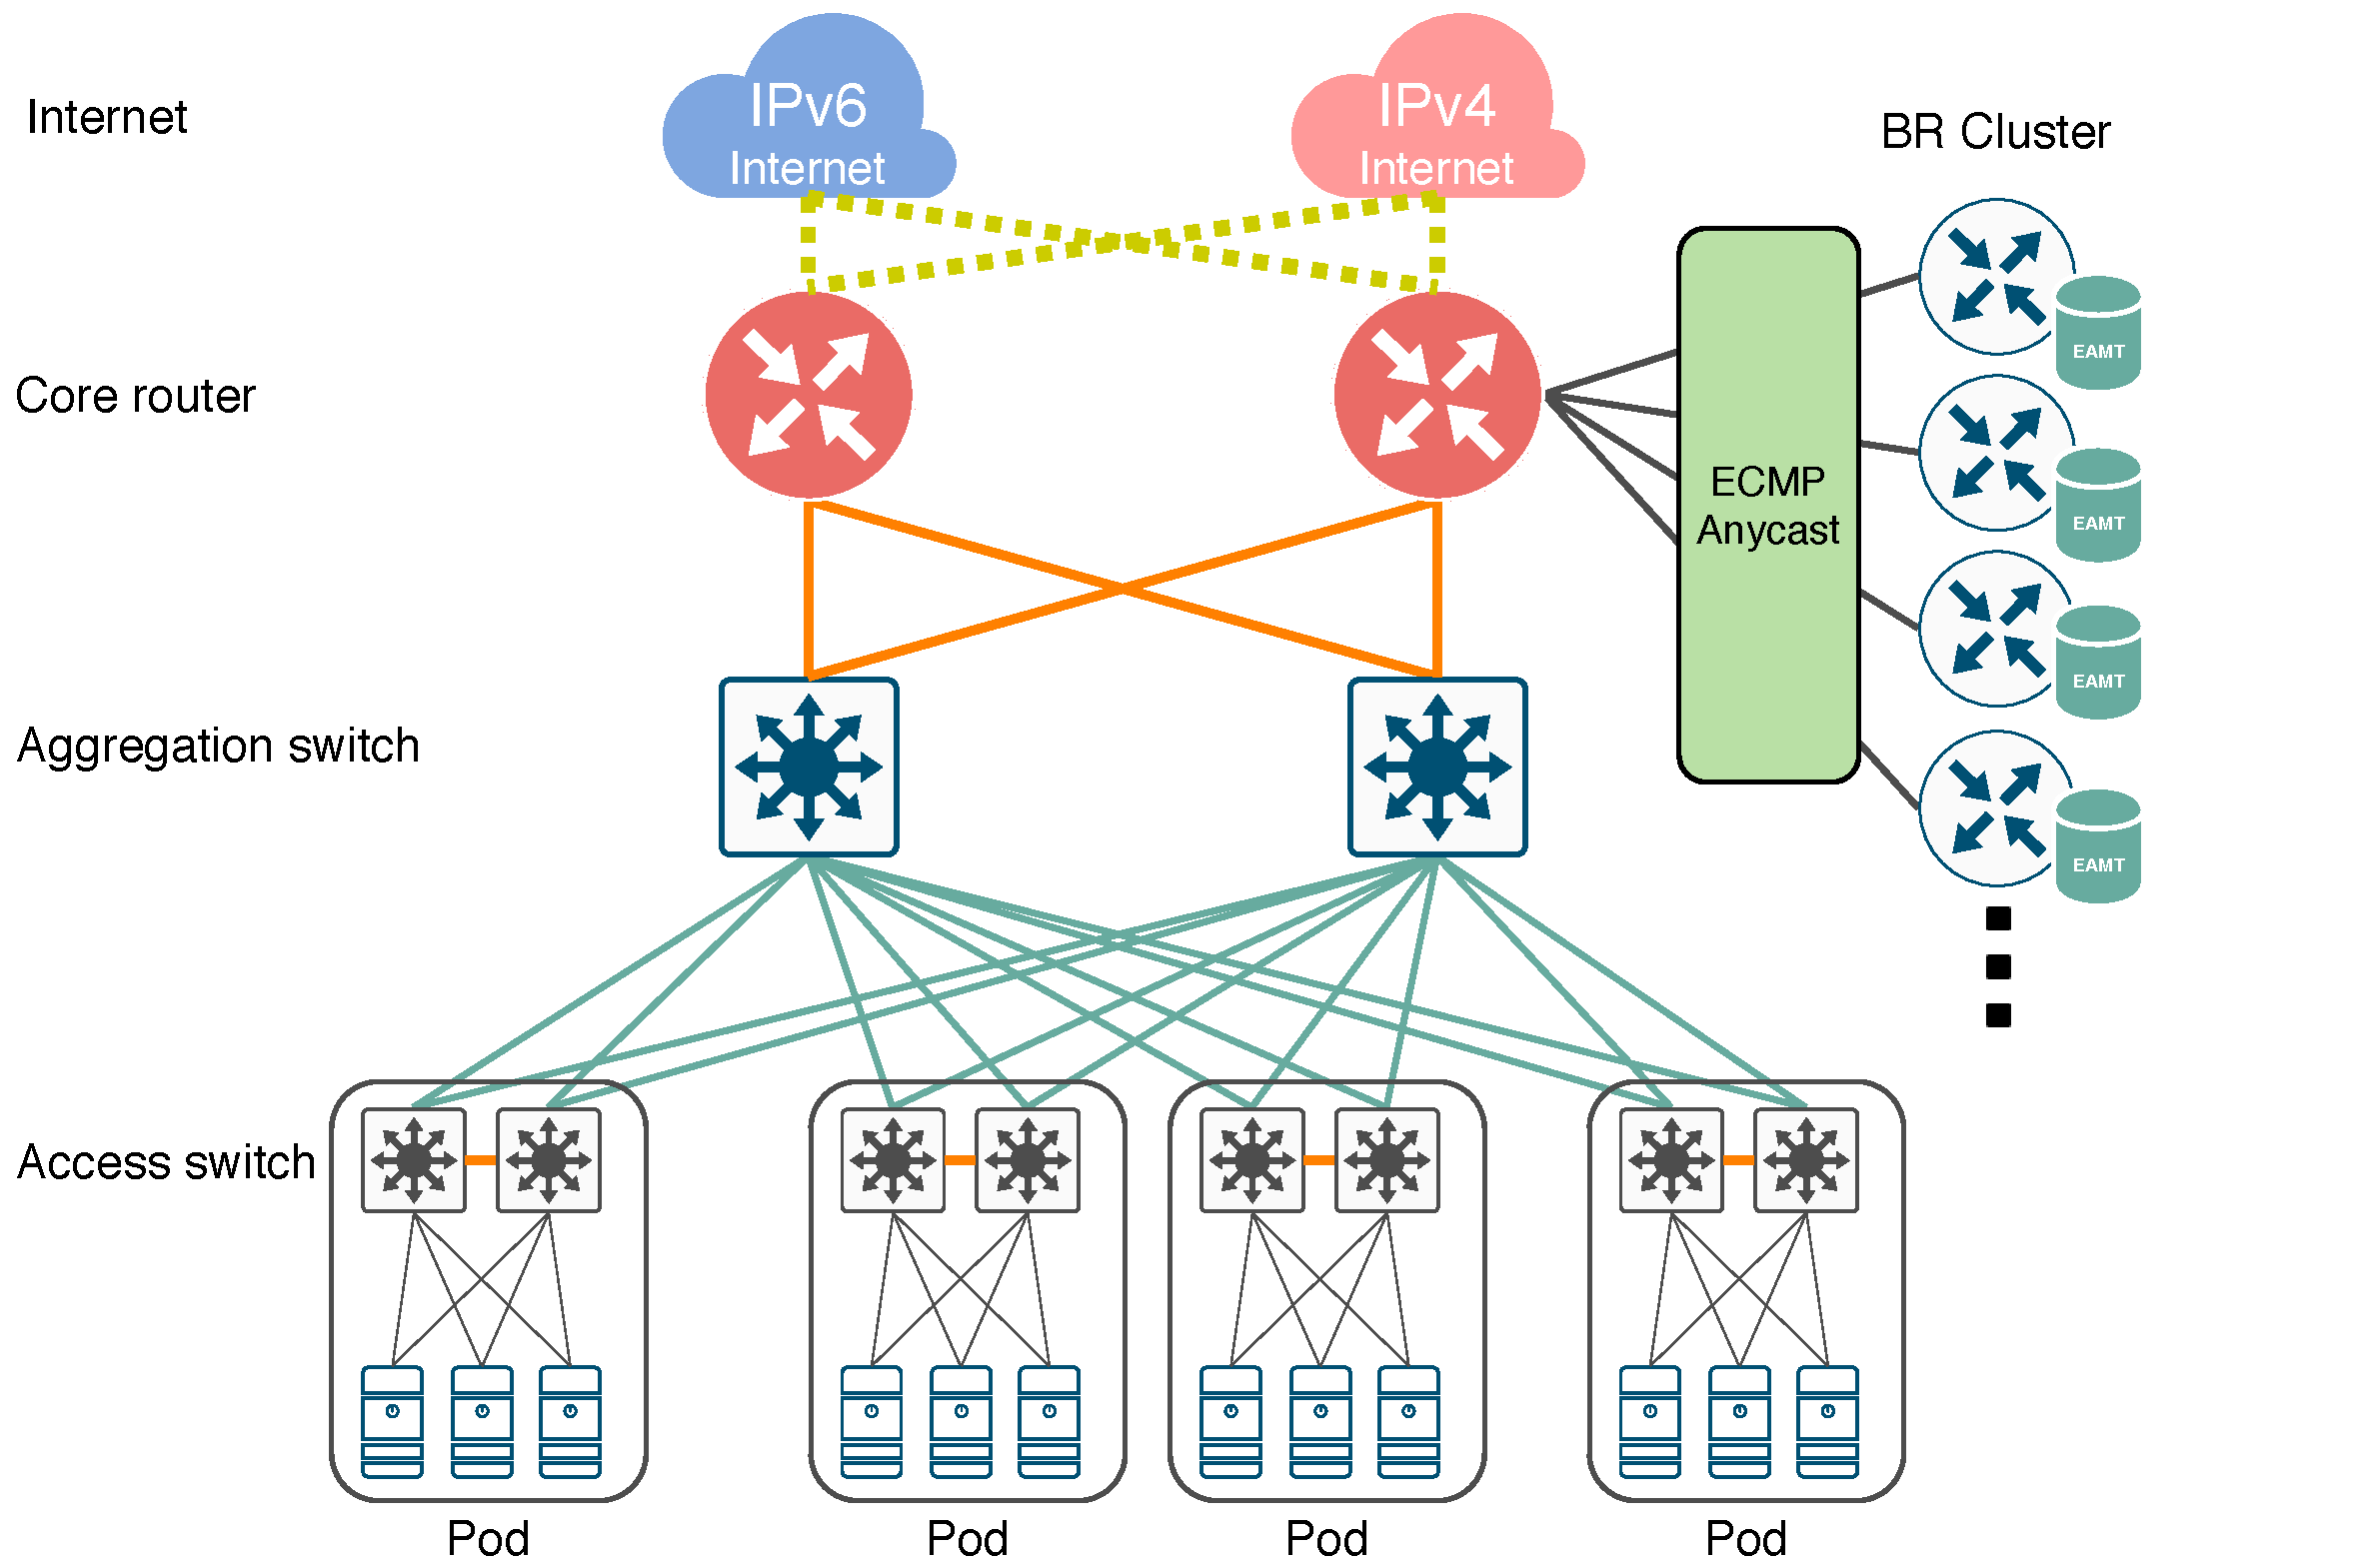
\includegraphics[width=12cm,pagebox=cropbox,clip]{img/siit-dc_scale.pdf}
%   \end{center}
%   \caption{BRを水平スケールすることが出来るSIIT-DCネットワーク}
%   \label{fig:siit-dc_network_scale}
% \end{figure}
% SIIT-DCの標準仕様\cite{RFC7755}では明示的に述べられていないが,本論文ではBRを並行して複数配置することで,スケールアウトが可能なネットワークデザインを立案する.
% 本ネットワークデザインでは,ECMP及びエニーキャスト\cite{RFC4786}を利用することにより,BRの数を水平に増加させることで,IPv4サービスの提供容量をリニアに増加させることが可能である.

% 図\ref{fig:siit-dc_network_scale}に本ネットワークデザインに則ってBR配置を行ったスケーラブルなSIIT-DCネットワークの例を示す.IPv4クライアントからのアクセスはいずれかのBRにフォワーディングされた後,IPv6プロトコルに変換された上で再度コアルータを介してIDCネットワーク内のIPv4サービス提供サーバに到達する.



% \subsection{基本的なパケットの流れ}
% \label{issue:siit-dc:packet_flow}

% \begin{figure}[h]
%     \begin{center}
%       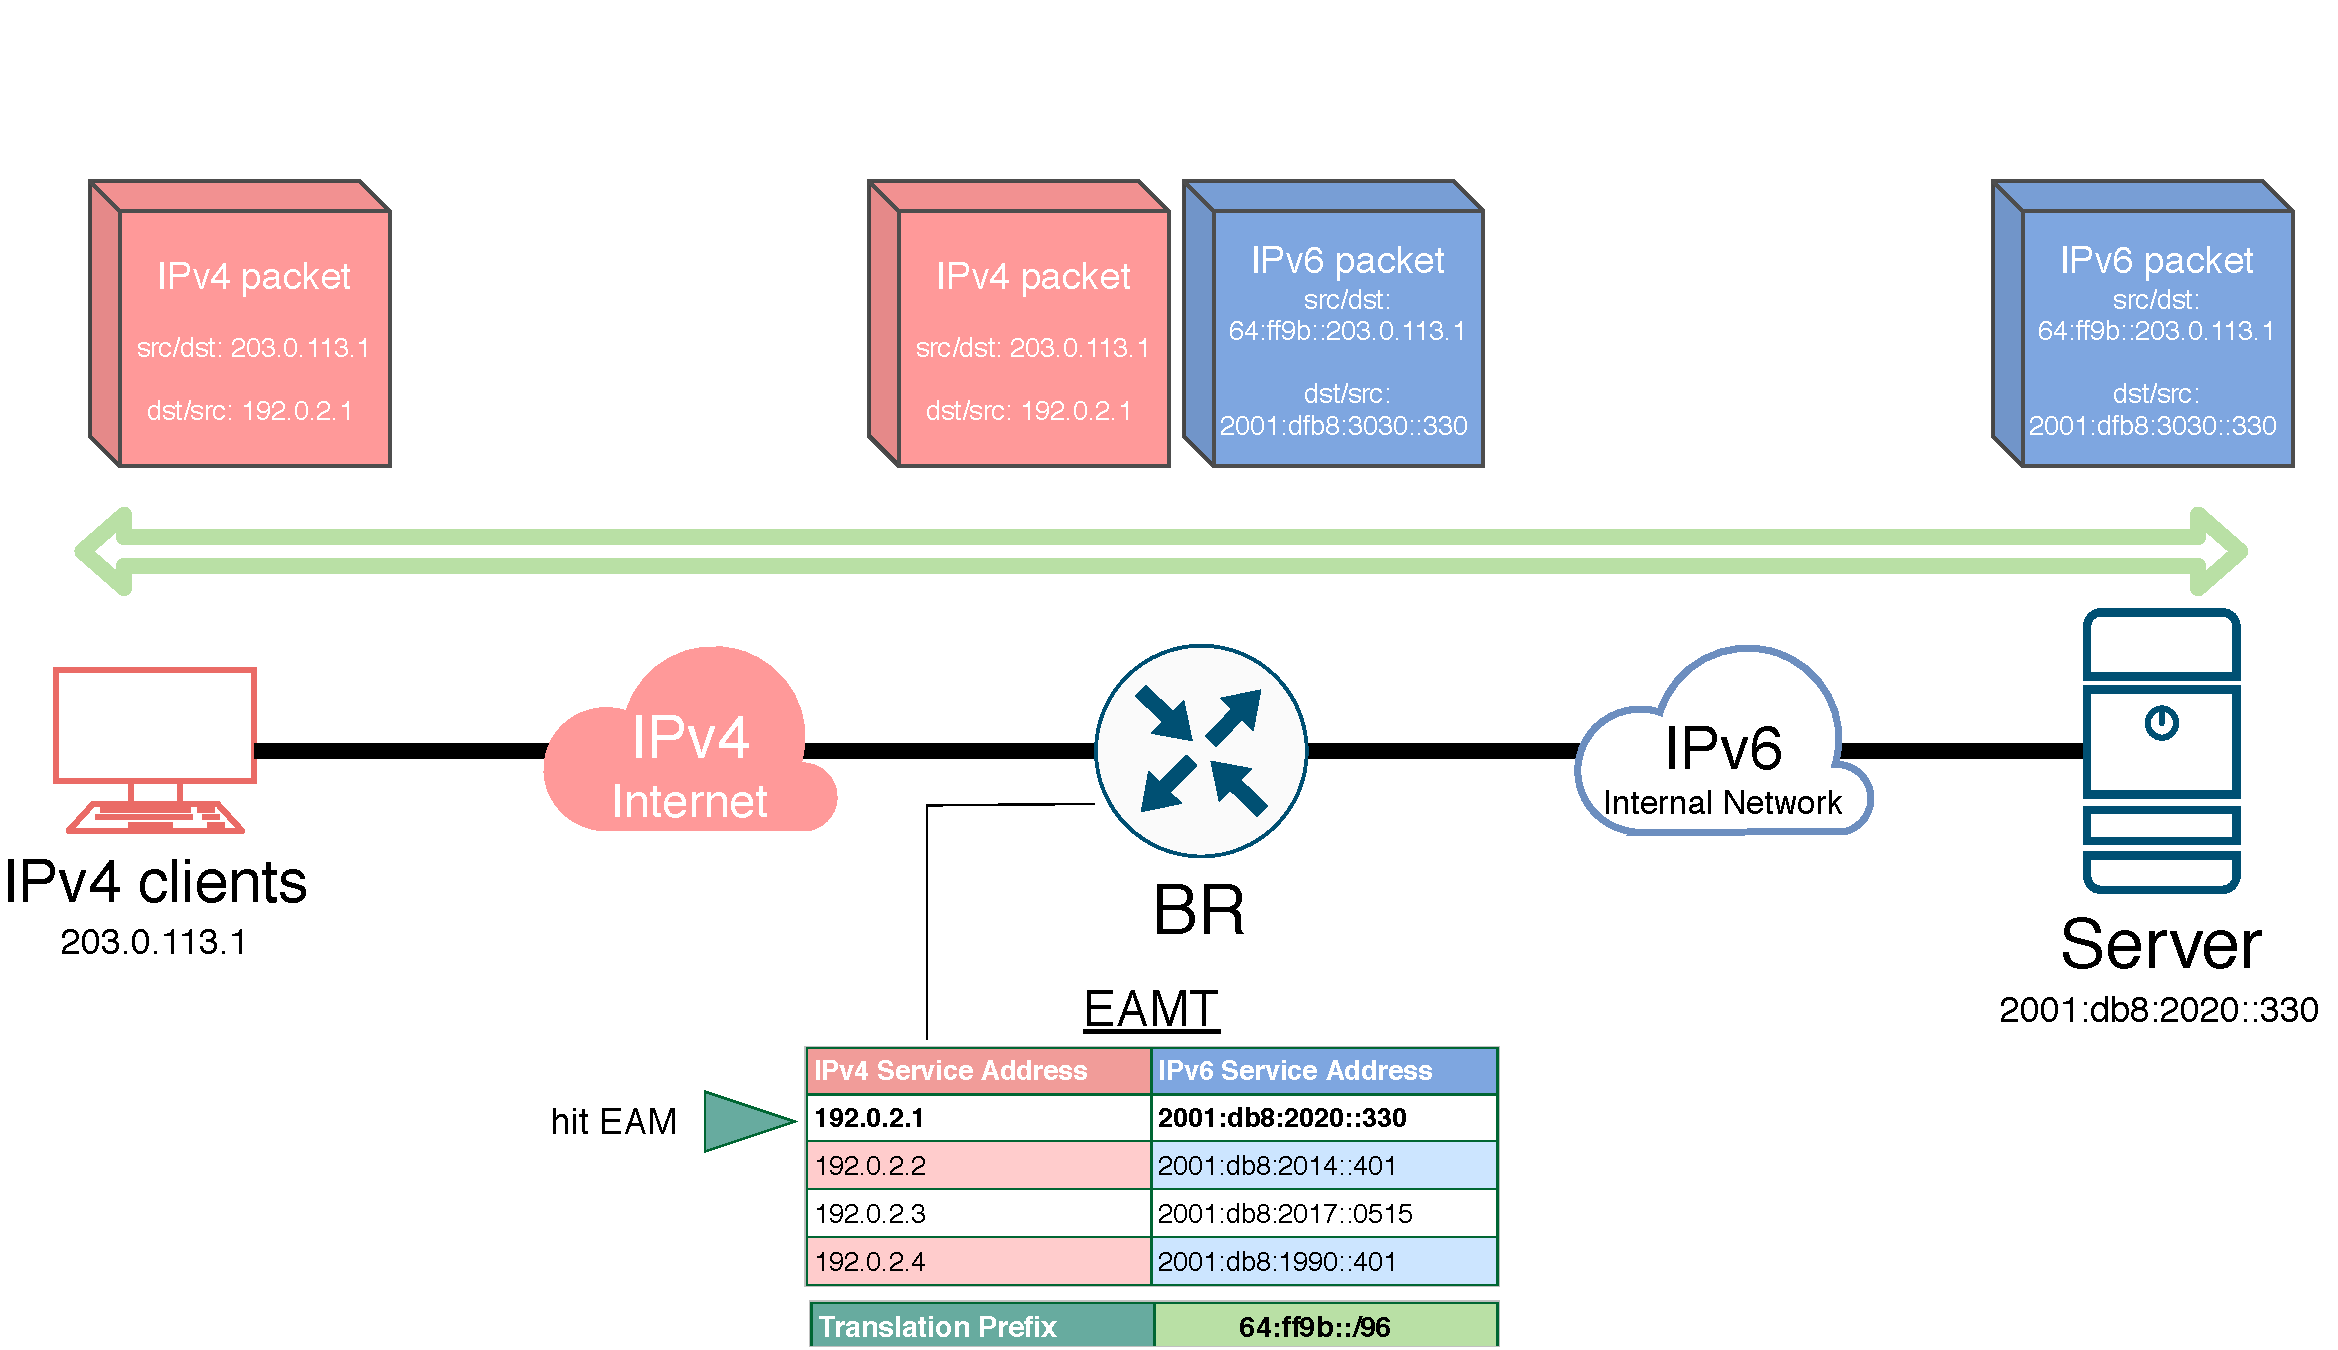
\includegraphics[width=14cm,pagebox=cropbox,clip]{img/siit-dc_packet.pdf}
%     \end{center}
%     \caption{SIIT-DC パケットの流れ}
%     \label{fig:siit-dc_packet}
% \end{figure}

% SIIT-DCにおける基本的なIPv4クライアントからのトラフィックの流れは以下の様になる.一連のパケットの送信元・送信先のアドレスの遷移を図\ref{fig:siit-dc_packet}に示す.

% IPv4クライアントのIPv4サービスアドレス宛のパケットはIPv4インターネットに接続するBRに到達後,当該BRが有するEAMTに従ってIPv6サービスアドレス宛のIPv6パケットに変換される.このパケットの送信元アドレスは変換プレフィックスに埋め込まれたIPv6アドレスとして表現される.IDC内のIPv6ネットワークを介してIPv6サーバに到達した後,IPv6サーバは送信元アドレスへの応答パケットを送信する.\ref{issue:siit-dc:translation-prefix}項で述べたように,変換プレフィックス宛のパケットはIPv6ネットワークを経由してBRにルーティングされる.IPv6サーバからの応答を受け取ったBRはEAMTを参照し,送信元アドレス(IPv6サービスアドレス)をIPv4サービスアドレスに書き換え,送信先アドレス(IPv4クライアントのIPv4アドレス)から変換プレフィックスを除去書き換えたのち,IPv4インターネットを介してIPv4クライアントに返送される.




% \section{SIIT-DCの課題}
% \label{issue:siit-dc_problems}
% 本節ではSIIT-DCの現状の課題及びそれに起因して起こる事象に関して述べる.

% \subsection{一貫したEAMTの必要性}
% \label{issue:siit-dc_problems:consistent}

% \begin{figure}[h]
%     \begin{center}
%       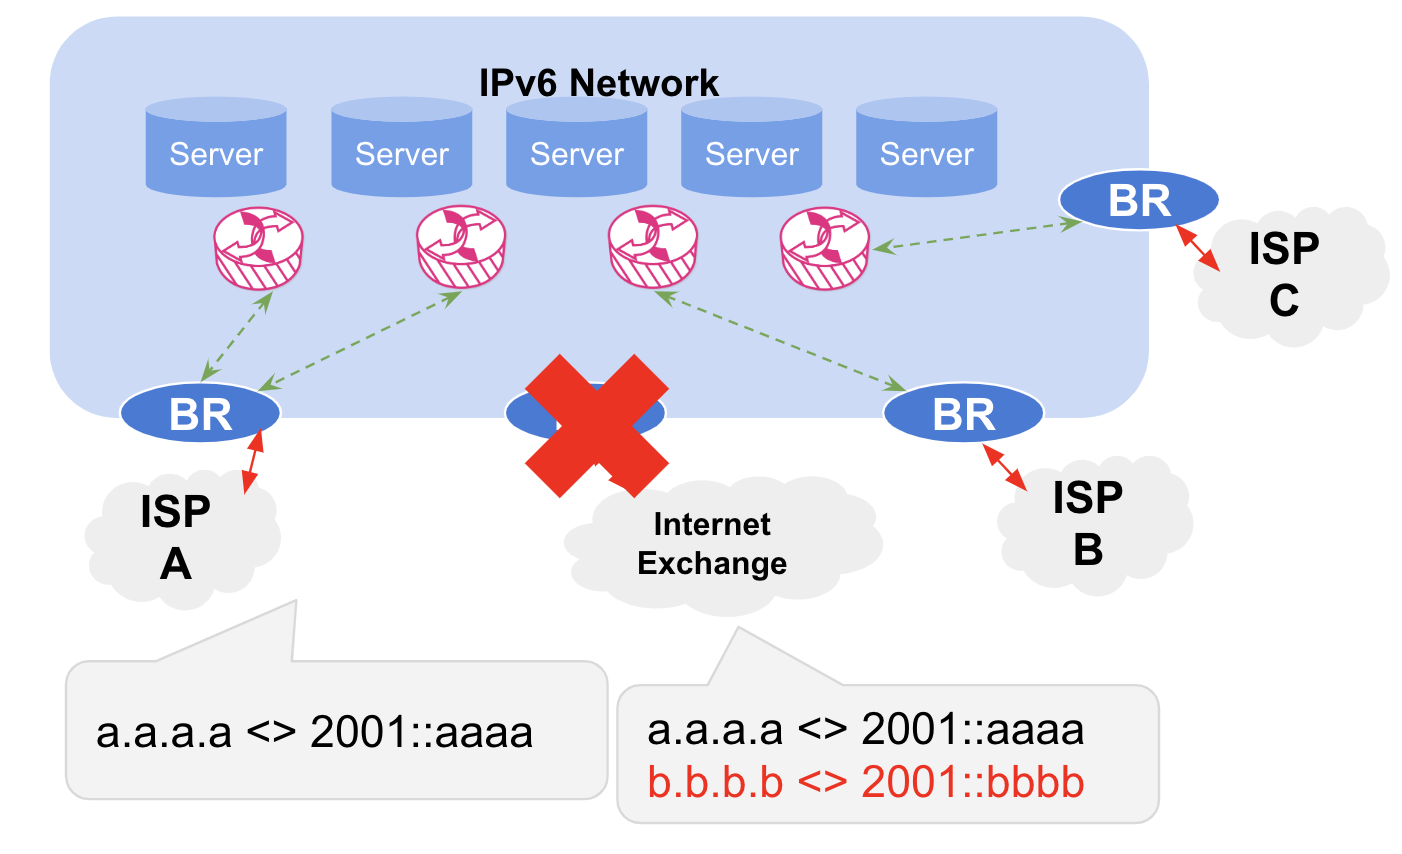
\includegraphics[width=10cm,pagebox=cropbox,clip]{img/siit-dc_can-not-failover.png}
%     \end{center}
%     \caption{BRに障害が発生した場合に適切にフェイルオーバーが出来ないケース}
%     \label{fig:siit-dc_can-not-failover}
% \end{figure}

% \ref{issue:siit-dc:terms}項で述べたように,SIIT-DCでは対外接続点ごとにBRを配置するネットワークデザインを採用することで,IPv6シングルスタックネットワークに最小限のIPv4ネットワークを追加するだけでIPv4サービスの提供を可能にしている.また\ref{issue:siit-dc:network}項や\ref{issue:siit-dc-merit:scalability}項で触れたように,複数のBRで共通した変換プレフィックスをエニーキャストでIDCネットワーク内に広告する運用を行うことにより,BR及び対外接続点の障害時に他のBRを用いてIPv4サービスの提供を継続することが出来る.この機構を有効に作用させるためには,SIIT-DCネットワーク内の全てのBRで一貫したEAMTの保持が求められる.

% しかしながら現状のSIIT-DC及びEAMTの仕様\cite{RFC7755,RFC7756,RFC7757}では,BRは他のBRとの間でEAMTを共有するためのメッセージング機構を有さない,これはBR間でEAMTの不一致が発生した場合に,差異となったEAMに該当するIPv4サービス宛のトラフィックを別のBRへ迂回出来なくなるケースが発生することを意味する.


% \subsection{変更追従性の欠如}
% \label{issue:siit-dc_problems:follow}

% \begin{figure}[h]
%     \begin{center}
%       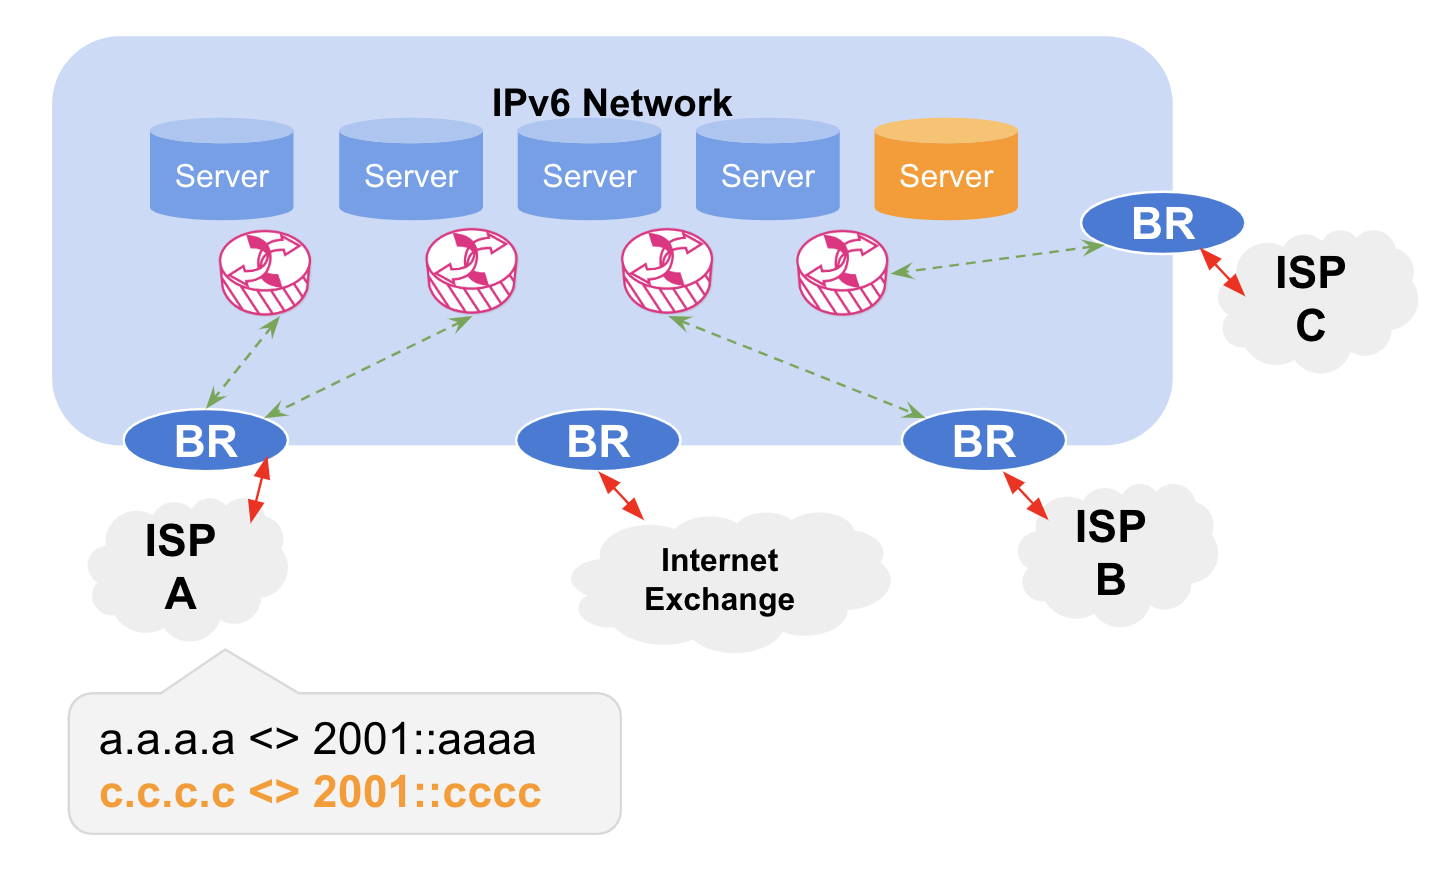
\includegraphics[width=10cm,pagebox=cropbox,clip]{img/siit-dc_add-server.png}
%     \end{center}
%     \caption{サーバを追加した際,全てのBRへの設定追加が必要になる.}
%     \label{fig:siit-dc_add-server}
% \end{figure}

% プライベートクラウド環境が一般的に利用されるIDCネットワークでは,日々多くのサーバやアプリケーションが追加・廃止・変更される.
% 一方で\ref{issue:siit-dc_problems:consistent}項で触れたように,SIIT-DCでIPv4提供サービスを冗長に運用するためには,IPv4提供サービスに該当するEAMがBRのEAMTに保持されることが要求される.IPv4提供サービスの構成に変更があった場合,全てのBRのEAMTを更新する必要がある.

% しかしながら現状SIIT-DC及びEAMTの仕様\cite{RFC7755,RFC7756,RFC7757}において,IPv4サービスを行うサーバの存在や状態によってダイナミックにEAMTを更新する機構は存在しない.そのため,IDCネットワークにおけるIGPなどによってIPv6サービスへの到達性が検証されていたとしても,IPv4サービスの場合はリアルタイムな構成変更に追従することが出来ない.


% \section{本章のまとめ}
% 第\ref{issue:siit-dc_problems}項で述べたように,現状のSIIT-DC及びEAMTの仕様はEAMTの一貫性を担保する手法の検討がなされておらず,それに起因した障害時の適切なフェイルオーバーの実行やIPv4サービスの増減時の変更追従に関しての課題がある.
% NPO日本ネットワークセキュリティ協会(JNSA)らの調査によればITシステムの障害の原因の約半数は人為ミスに分類されるものにあり\cite{human_error},サービスの安定的な稼働を実現するためには単調な繰り返し動作を含む運用をシステムによって減らす必要がある.


%%% Local Variables:
%%% mode: japanese-latex
%%% TeX-master: "./thesis"
%%% End:
